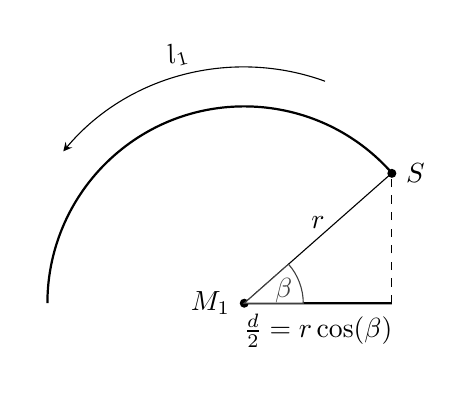
\begin{tikzpicture}[
    scale=2.5,
    >=stealth,
    point/.style = {draw, circle,  fill = black, inner sep = 1pt},
    dot/.style   = {draw, circle,  fill = black, inner sep = .2pt},
  ]
    \clip (-0.1,0.6) rectangle (2,2.4);
	\coordinate (R1) at (1,1); % Mittelpunkt des ersten Kreises
	\coordinate (R2) at (2.5,1); % Mittelpunkt des zweiten Kreises
	
	% Kreismittelpunkte
	\node (M1) at (R1) [point, label = {left:$M_1$}]{};
	\node (M2) at (R2) [point, label = {below:$M_2$}]{};
	
	% Bögen
	\draw[thick] (R1) ++(41.41:1) arc (41.41:180:1);
	%\draw[dashed] (R1) ++(-41.41:1) arc (-41.41:41.41:1);
	%\draw[thick] (R2) ++(221.41:1) arc (221.41:498.59:1);
	%\draw[dashed] (R2) ++(138.59:1) arc (138.59:221.41:1);
	
	% Radius und Abstand der Kreise einzeichnen
	\draw[thick] (R1) -- node [below] {$\frac{d}{2}=r\cos(\beta)$} (1.75,1);
	\draw (R1) -- node [above] {$r$} +(41.41:1);
	\draw[dashed] (1.75,1) -- +(0,0.66);
	\filldraw[fill=white,draw=gray!50!black] (R1) -- (1.3,1)
            arc [start angle=0, end angle=41.41, radius=0.3] -- cycle;
    \draw (1.2,1.065) node[gray!50!black] {$\beta$};
	
	% Schnittpunkt des Kreises
	\node (S) at (1.75,1.66) [point, label = right:$S$] {};
	
	\draw[->] (R1) ++(70:1.2) arc (70:140:1.2) node[midway, sloped, above]{$l_1$};
	
\end{tikzpicture}